\documentclass{standalone}
\usepackage{tikz}
\usepackage{ctex,siunitx,bm}
\setCJKmainfont{Noto Serif CJK SC}
\usepackage{tkz-euclide,ninecolors}
\usepackage{amsmath}
\usetikzlibrary{patterns, calc}
\usetikzlibrary {decorations.pathmorphing, decorations.pathreplacing, decorations.shapes,decorations.markings}
\begin{document}
\small
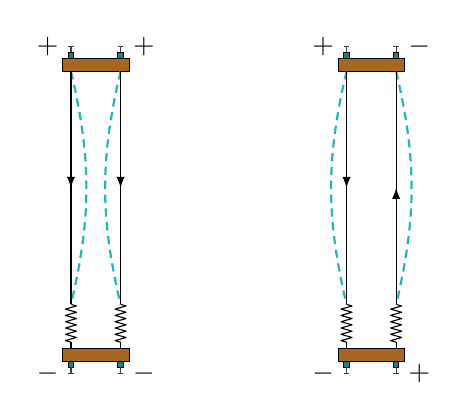
\begin{tikzpicture}[>=latex,yscale=0.8,xscale=0.7]
  \draw[very thin,fill=brown5] (-0.6,-2.4)rectangle(0.6,-2.2)(-0.6,2.4)rectangle(0.6,2.2);
  \foreach \x in {-0.45,0.45}
  {
    \draw(\x,-2.2)--(\x,-2.1);
    \foreach \y in {-2.1,-2.0,...,-1.5}
    {\draw [line join=round](\x,\y)--++(-0.1,0.025)--++(0.2,0.05)--++(-0.1,0.025);}
    \draw[fill=cyan5] (\x+0.05,2.4)rectangle(\x-0.05,2.5);
    \draw[darkgray] (\x,2.5)--++(0,0.1);
    \draw[darkgray] (\x-0.05,2.6)--++(0.1,0);
    \draw[fill=cyan5] (\x+0.05,-2.4)rectangle(\x-0.05,-2.5);
    \draw[darkgray] (\x,-2.5)--++(0,-0.1);
    \draw[darkgray] (\x-0.05,-2.6)--++(0.1,0);
  }
  \draw[cyan7,thick,densely dashed](-0.45,2.2)to[bend left=15](-0.45,-1.5);
  \draw[cyan7,thick,densely dashed](0.45,2.2)to[bend right=15](0.45,-1.5);
  \draw[postaction={decorate},decoration={markings,mark={at position 0.5 with {\arrow{>}}}}](-0.45,2.2)--(-0.45,-1.5);
  \draw[postaction={decorate},decoration={markings,mark={at position 0.5 with {\arrow{>}}}}](0.45,2.2)--(0.45,-1.5);
  \node at (-0.5, 2.6) [left] {$+$};
  \node at ( 0.5, 2.6) [right] {$+$};
  \node at (-0.5,-2.6) [left] {$-$};
  \node at ( 0.5,-2.6) [right] {$-$};
  \begin{scope}[xshift=5cm]
    \draw[very thin,fill=brown5] (-0.6,-2.4)rectangle(0.6,-2.2)(-0.6,2.4)rectangle(0.6,2.2);
  \foreach \x in {-0.45,0.45}
  {
    \draw(\x,-2.2)--(\x,-2.1);
    \foreach \y in {-2.1,-2.0,...,-1.5}
    {\draw [line join=round](\x,\y)--++(-0.1,0.025)--++(0.2,0.05)--++(-0.1,0.025);}
    \draw[fill=cyan5] (\x+0.05,2.4)rectangle(\x-0.05,2.5);
    \draw[darkgray] (\x,2.5)--++(0,0.1);
    \draw[darkgray] (\x-0.05,2.6)--++(0.1,0);
    \draw[fill=cyan5] (\x+0.05,-2.4)rectangle(\x-0.05,-2.5);
    \draw[darkgray] (\x,-2.5)--++(0,-0.1);
    \draw[darkgray] (\x-0.05,-2.6)--++(0.1,0);
  }
  \draw[cyan7,thick,densely dashed](-0.45,2.2)to[bend right=15](-0.45,-1.5);
  \draw[cyan7,thick,densely dashed](0.45,2.2)to[bend left=15](0.45,-1.5);
  \draw[postaction={decorate},decoration={markings,mark={at position 0.5 with {\arrow{>}}}}](-0.45,2.2)--(-0.45,-1.5);
  \draw[postaction={decorate},decoration={markings,mark={at position 0.5 with {\arrow{>}}}}](0.45,-1.5)--(0.45,2.2);
  \node at (-0.5, 2.6) [left] {$+$};
  \node at ( 0.5, 2.6) [right] {$-$};
  \node at (-0.5,-2.6) [left] {$-$};
  \node at ( 0.5,-2.6) [right] {$+$};
  \end{scope}
\end{tikzpicture}
\end{document}